\documentclass[11pt,a4,table]{article}

\renewcommand{\footnotesize}{\fontsize{9pt}{11pt}\selectfont}

%%%%%%%%%%%%%%%%%%%%%%%%%%%%%%%%%%%%%%%%%%%%%%%%%%%%

% Page Dimensions
\usepackage[top=1.0in, bottom=1.0in, left= 0.80in, right=0.80in]{geometry}

%%%%%%%%%%%%%%%%%%%%%%%%%%%%%%%%%%%%%%%%%%%%%%%%%%%%

% Caption options
\usepackage[margin= 16pt , footnotesize ,  sc , labelfont=bf , labelsep=period , format=plain , justification=centerfirst]{caption}


%%%%%%%%%%%%%%%%%%%%%%%%%%%%%%%%%%%%%%%%%%%%%%%%%%%%
%load minimum set of other required packages
\usepackage{amsfonts}
\usepackage{amsmath}
\usepackage{amssymb}
\usepackage{amsthm}
\usepackage{array}
\usepackage{bbm}
\usepackage{booktabs,longtable}
\usepackage{eurosym}
\usepackage{floatrow}
\usepackage{graphicx}
\usepackage{hyperref}
\usepackage{harvard}
\usepackage[english]{babel}
\usepackage{multirow}
\usepackage{lscape}
\usepackage{pdflscape}
\usepackage{rotating}
\usepackage{subfig}
\usepackage{setspace}
\usepackage{titlesec}
\usepackage{verbatim}
\usepackage{xcolor}
\usepackage[T1]{fontenc}

\usepackage[utf8]{inputenc}


%%%%%%%%%%%%%%%%%%%%%%%%%%%%%%%%%%%%%%%%%%%%%%%%%%%%
%%%%%%%%%%%%%%%%%%%%%%%%%%%%%%%%%%%%%%%%%%%%%%%%%%%%%

% and tikz
\usepackage{tikz}
\usetikzlibrary{decorations.pathreplacing}
	\definecolor{cinnabar}{rgb}{0.89, 0.26, 0.2}
	\definecolor{ceruleanblue}{rgb}{0.16, 0.32, 0.75}

\usetikzlibrary{patterns}
\usetikzlibrary{matrix}
\usetikzlibrary{arrows,backgrounds,decorations}

\newcommand*\circled[1]{\tikz[baseline=(char.base)]{
            \node[shape=circle,draw,inner sep=2pt] (char) {#1};}}
            
% and optimally spaces tables

\usepackage{tabularx, booktabs}
\newcolumntype{Y}{>{\centering\arraybackslash}X}


%%%%%%%%%%%%%%%%%%%%%%%%%%%%%%%%%%%%%%%%%%%%%%%%%%%%

%% Roman numerals command thing.
\makeatletter
\newcommand{\rmnum}[1]{\romannumeral #1}
\newcommand{\Rmnum}[1]{\expandafter\@slowromancap\romannumeral #1@}
\makeatother

%%%%%%%%%%%%%%%%%%%%%%%%%%%%%%%%%%%%%%%%%%%%%%%%%%%%

% fake section command
\newcommand{\fakesection}[1]{%
  \par\refstepcounter{section}% Increase section counter
  \sectionmark{#1}% Add section mark (header)
  \addcontentsline{toc}{section}{\protect\numberline{\thesection}#1}% Add section to ToC
  % Add more content here, if needed.
}


%%%%%%%%%%%%%%%%%%%%%%%%%%%%%%%%%%%%%%%%%%%%%%%%%%%%

%% ------------------------------------------
%% Journal of Finance conventions
%% ------------------------------------------

\renewcommand{\thesection}{\Roman{section}}
\renewcommand{\thesubsection}{\Alph{subsection}}
\renewcommand{\thetable}{\Roman{table}}
\renewcommand{\abstractname}{\textsc{ABSTRACT}}
\makeatletter
\renewcommand{\baselinestretch}{1.10}
\renewcommand{\topfraction}{0.99}
\renewcommand{\bottomfraction}{0.99}
\setcounter{topnumber}{2}
\setcounter{bottomnumber}{2}
\setcounter{totalnumber}{4}
\setcounter{dbltopnumber}{2}
\renewcommand{\dbltopfraction}{0.9}
\renewcommand{\textfraction}{0.07}
\renewcommand{\floatpagefraction}{0.9}
\renewcommand{\dblfloatpagefraction}{0.9}
\titleformat{\section}{\centering\large\bfseries}{\thesection.}{1em}{}
\titleformat{\subsection}{\normalsize\itshape}{\thesubsection.}{1em}{}
\titleformat{\subsubsection}{\normalsize\itshape}{\thesubsubsection.}{1em}{}


%%%%%%%%%%%%%%%%%%%%%%%%%%%%

% math shocks cuts, theorems, lemmas etc.
\newcommand{\inner}[2]{\left < #1 \big | #2 \right >}
\newcommand{\proj}[2]{\mbox{proj} \left ( #1 \big | #2 \right )}
\newcommand{\cov}[2]{\mbox{cov}\left (#1 ,#2 \right )}
\newcommand{\var}[1]{\mbox{var}[#1]}
\newcommand{\Gray}[1]{{\color{gray}#1}}
\newcommand{\Red}[1]{{\color{red}#1}}


\newtheorem{theorem}{Theorem}
\newtheorem{acknowledgement}{Acknowledgement}
\newtheorem{algorithm}{Algorithm}
\newtheorem{axiom}{Axiom}
\newtheorem{case}{Case}
\newtheorem{claim}{Claim}
\newtheorem{conclusion}{Conclusion}
\newtheorem{condition}{Condition}
\newtheorem{conjecture}{Conjecture}
\newtheorem{corollary}{Corollary}
\newtheorem{criterion}{Criterion}
\newtheorem{definition}{Definition}
\newtheorem{example}{Example}
\newtheorem{exercise}{Exercise}
\newtheorem{lemma}{Lemma}
\newtheorem{notation}{Notation}
\newtheorem{problem}{Problem}
\newtheorem{proposition}{Proposition}
\newtheorem{hypothesis}{Hypothesis}
\newtheorem{remark}{Remark}
\newtheorem{solution}{Solution}
\newtheorem{summary}{Summary}

%%%%%%%%%%%%%%%%%%%%%%%%%%%%%%%%%%%%%%%%%%%%%%%%%%%%

% and choose line spacing (comes from setspace)

%\singlespacing
%\onehalfspacing
%\doublespacing
%\setstretch{1.5}
%\setstretch{2}

% make quote right flushed.
\makeatletter{}
\g@addto@macro\quote\flushright
\makeatother


%%%%%%%%%%%%%%%%%%%%%%%%%%%%%%%%%%%%%%%%%%%%%%%%%%%%%%%%%%%%%%%%%%%%%%
%%%%%%%%%%%%%%%%%%%%%%%%%%%%%%%%%%%%%%%%%%%%%%%%%%%%%%%%%%%%%%%%%%%%%%


\begin{document}

\vspace*{-0.7in}

\begin{center}
 \textbf{Continuous Time Finance: Solution Problem Set 2} \\
Ilaria Piatti 
\end{center} 


\begin{enumerate}
    \item Consider a two periods binomial model with parameters $r=0.25, u=1/d=2$ and $S_0=4$:
    
    \begin{enumerate}
        \item Compute the price of a European call option with strike price $K=5$ and maturity $T=2$. The possible stock prices at the end of period 2 are 16, 4 and 1, and the corresponding payoffs of the call option are 11, 0 and 0.
        \begin{figure}[hp]
        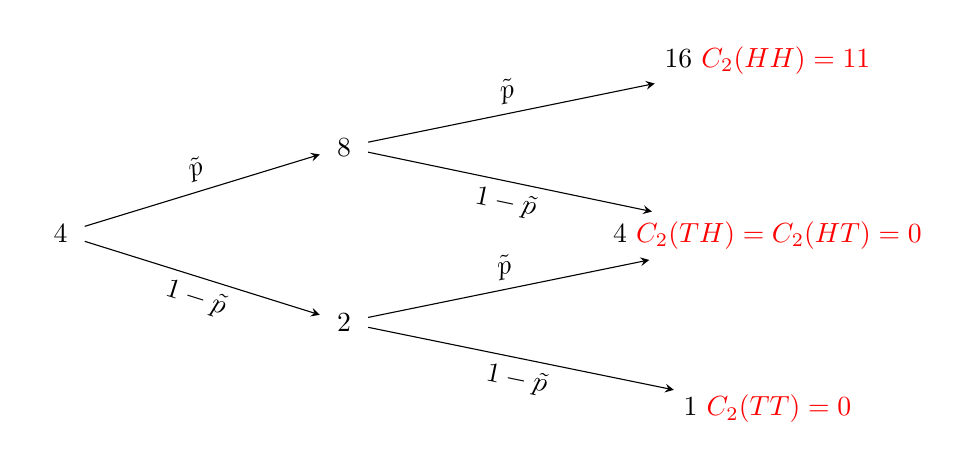
\begin{tikzpicture}[>=stealth , sloped , scale = 0.6] 
            \matrix (tree) [%
              matrix of nodes,
              minimum size=0.6cm,
              column sep=3.00cm,
              row sep=0.5cm,
              ampersand replacement=\&
            ]
                  {
                  	\&   	\& $16$    \textcolor{red}{$C_2(HH) = 11$} \\
                  	\& $8$ 	\&                                    \\
              $4$ 	\&   	\& $4$     \textcolor{red}{$C_2(TH)=C_2(HT) = 0$} \\
                  	\& $2$ 	\&                                    \\
                  	\&   	\& $1$     \textcolor{red}{$C_2(TT) = 0$} \\
            };
            \draw[->] (tree-3-1) -- (tree-2-2) node [midway,above]{$\Tilde{p}$} ;
            \draw[->] (tree-3-1) -- (tree-4-2) node [midway,below]{$1-\Tilde{p}$} ;
            \draw[->] (tree-2-2) -- (tree-1-3) node [midway,above]{$\Tilde{p}$} ;
            \draw[->] (tree-2-2) -- (tree-3-3) node [midway,below]{$1-\Tilde{p}$} ;
            \draw[->] (tree-4-2) -- (tree-3-3) node [midway,above]{$\Tilde{p}$} ;
            \draw[->] (tree-4-2) -- (tree-5-3) node [midway,below]{$1-\Tilde{p}$} ;
        \end{tikzpicture}
        \end{figure}
        
        The risk-neutral probability of an upward stock price move, $\Tilde{p}$, is given by
        \begin{equation*}
            \Tilde{p}=\frac{1+r-d}{u-d} = \frac{1+0.25-0.5}{2-0.5}=0.5.
        \end{equation*}
        Therefore, using the risk neutral valuation forula,
        \begin{align*}
            C_1(H) &=\frac{1}{1+0.25}(11\cdot 0.5 + 0\cdot 0.5) = 4.4,\\
            C_1(T) &=\frac{1}{1+0.25}(0\cdot 0.5 + 0\cdot 0.5) = 0.
        \end{align*}
        and
        \begin{equation*}
            C_0 = \frac{1}{1+0.25}4.4\cdot 0.5 = 1.76.
        \end{equation*}
    \end{enumerate}

    Consider now a European lookback option with a payoff at maturity $V_T$ given by:
    \begin{equation*}
        V_T=\max_{k=0,1,2}(S_k-K)^+,
    \end{equation*}
    where $K=5$, as in point (a) above.
    
    \begin{enumerate}
        \setcounter{enumii}{1}
    
        \item Compute for every trajectory of the binomial tree the corresponding value of $V_T$. Compare the results with the standard case of a European call option. Do you see any differences?\\
        The values of the European lookback option at maturity $T=2$ are: $V_2(HH)=11, V_2(HT)=3, V_2(TH)=0$, and $V_2(TT)=0$. The probability of having a positive cashflow is higher with the lookback option with respect to the standard cell option, so the expected value of the option is bigger.
    
        \item Compute the quantities $\Delta_1$ and $\Delta_0$ which correspond to the \textit{delta} hedging factors for the lookback option.\\
        At time 1, the deltas of the hedging portfolio for each node are given by:
        \begin{align*}
            \Delta_1(H) &= \frac{11-3}{16-4} = \frac{2}{3},\\
            \Delta_1(T) &= \frac{0}{4-1} = 0.
        \end{align*}
        Using the risk neutral valuation formula, the value of the option at time 1 is given by:
        \begin{align*}
            V_1(H) &= \frac{1}{1+0.25}(11\cdot 0.5 + 3\cdot 0.5)= 5.6,\\
            V_1(T) &= \frac{1}{1+0.25}(0\cdot 0.5 + 0\cdot 0.5) = 0.
        \end{align*}
        Therefore, the delta of the hedging portfolio at time 0 is:
        \begin{equation*}
            \Delta_0 = \frac{5.6-0}{8-2}\cong 0.93.
        \end{equation*}
        
        \item By means of the risk-neutral valuation principle determine the price at $t=0$ of the lookback option.\\
        The price of the lookback option at time 0 is
        \begin{equation*}
            V_0 = \frac{1}{1+0.25}(5.6\cdot 0.5 + 0\cdot 0.5) = 2.24.
        \end{equation*}
    \end{enumerate}
    
    
    \item Consider a \textit{n} periods binomial model with parameters $r=0.25, u=1/d=2$ and $S_0=4$. An European (American) put option with maturity $T$ and exercise price $K$ is the right, but not the obligation to sell at date $T$ (or at one date $t\in(0,...,T)$) the underlying stock for a price equal to $K$.
    
    \begin{enumerate}
        \item Explain why the payoff $p_T$ at maturity of a European put option is given by
        \begin{equation*}
            p_T=(K-S_T)^+.
        \end{equation*}
        At maturity we will exercise the right to sell the stock for a price equal to $K$ only if the stock price on the market is lower than $K$, i.e. $S_T < K$. If this is the case, the payoff of the option is given by the difference $K-S_T$. If the market price at maturity, $S_T$, is higher than the exercise price $K$, the option is not exercised and the payoff is zero. In short,
        \begin{equation*}
            p_T=    \begin{cases}
                        K-S_T   & \text{if $S_T < K$} \\
                        0       & \text{if $S_T \geq K$}
                    \end{cases},       
        \end{equation*}
        Which can also be written as the positive part of $K-S_T$, i.e. $p_T=(K-S_T)^+$.
        
\newpage
        \item Compute the price $p_0$ at $t=0$ of a European put with parameters $T=1$ and $K=5$ in the binomial model.
        \begin{figure}[hp]
        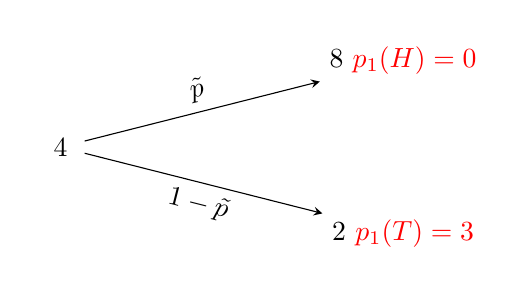
\begin{tikzpicture}[>=stealth , sloped , scale = 0.6] 
            \matrix (tree) [%
              matrix of nodes,
              minimum size=0.6cm,
              column sep=3.00cm,
              row sep=0.5cm,
              ampersand replacement=\&
            ]
                  {
                  	\& $8$ 	\textcolor{red}{$p_1(H)=0$} \\
              $4$ 	\&   	                            \\
                  	\& $2$ 	\textcolor{red}{$p_1(T)=3$} \\
            };
            \draw[->] (tree-2-1) -- (tree-1-2) node [midway,above]{$\Tilde{p}$} ;
            \draw[->] (tree-2-1) -- (tree-3-2) node [midway,below]{$1-\Tilde{p}$} ;
        \end{tikzpicture}
        \end{figure}\\
        The risk neutral probability $\Tilde{p}$ is given by
        \begin{equation*}
            \Tilde{p} = \frac{1+r-d}{u-d} = \frac{1+0.25-0.5}{2-0.5} = 0.5.
        \end{equation*}
        Therefore, using the risk neutral valuation formula,
        \begin{equation*}
            p_0 = \frac{1}{1+0.25}(0\cdot 0.5 + 3\cdot 0.5)=1.2.
        \end{equation*}
        
        \item Compute the price $P_0$ of an American put option in a binomial model with parameters $T=1$ and $K=5$. First motivate the following equality:
        \begin{equation*}
            P_0=\max\{p_0,(K-S_0)^+\}.
        \end{equation*}
        $P_0 = \max\{p_0,(K-S_0)^+\}$ because if $(K-S_0)^+$, which is the value of exercising the option at time $t=0$, is higher than the value at time zero of a corresponding European option $p_0$, we will exercise the American option at time 0, while if $p_0>(K-S_0)^+$ we will not exercise at time zero (before maturity) and the American option is equivalent to a European option, i.e. $P_0 = p_0$.\\
        In this case, $(K-S_0)^+=1<p_0 = 1.2$. Therefore, the American option is not exercised before maturity and its time-0 price is $P_0=p_0=1.2$.
        
        
        \item Compute the price $p_0$ of a European put option in a binomial model with parameters $T=2$ and $K=5$ by first determining the corresponding hedging strategy.
        \begin{figure}[hp]
        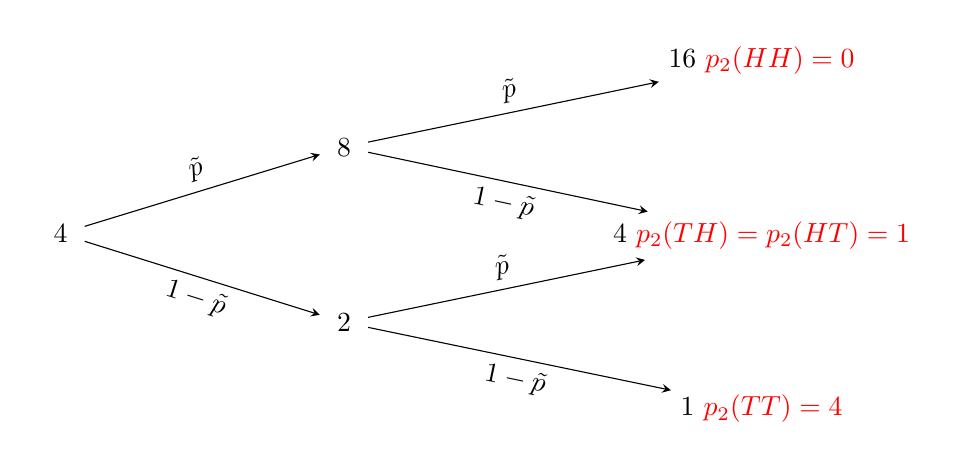
\begin{tikzpicture}[>=stealth , sloped , scale = 0.6] 
            \matrix (tree) [%
              matrix of nodes,
              minimum size=0.6cm,
              column sep=3.00cm,
              row sep=0.5cm,
              ampersand replacement=\&
            ]
                  {
                  	\&   	\& $16$    \textcolor{red}{$p_2(HH) = 0$} \\
                  	\& $8$ 	\&                                    \\
              $4$ 	\&   	\& $4$     \textcolor{red}{$p_2(TH)=p_2(HT) = 1$} \\
                  	\& $2$ 	\&                                    \\
                  	\&   	\& $1$     \textcolor{red}{$p_2(TT) = 4$} \\
            };
            \draw[->] (tree-3-1) -- (tree-2-2) node [midway,above]{$\Tilde{p}$} ;
            \draw[->] (tree-3-1) -- (tree-4-2) node [midway,below]{$1-\Tilde{p}$} ;
            \draw[->] (tree-2-2) -- (tree-1-3) node [midway,above]{$\Tilde{p}$} ;
            \draw[->] (tree-2-2) -- (tree-3-3) node [midway,below]{$1-\Tilde{p}$} ;
            \draw[->] (tree-4-2) -- (tree-3-3) node [midway,above]{$\Tilde{p}$} ;
            \draw[->] (tree-4-2) -- (tree-5-3) node [midway,below]{$1-\Tilde{p}$} ;
        \end{tikzpicture}
        \end{figure}
        \\
        At time 1, the deltas of the hedging portfolio for each node are given by:
        \begin{align*}
            \Delta_1(H) &= \frac{0-1}{16-4} = - \frac{1}{12},\\
            \Delta_1(T) &= \frac{1-4}{4-1} = -1.
        \end{align*}
        Using the risk neutral valuation formula, the value of the European put option at time 1 is given by:
        \begin{align*}
            p_1(H) &= \frac{1}{1+0.25}(0\cdot 0.5 + 1\cdot 0.5) = 0.4,\\
            p_1(T) &= \frac{1}{1+0.25}(1\cdot 0.5 + 4\cdot 0.5) = 2.
        \end{align*}
        Therefore, the delta of the hedging portfolio at time 0 is:
        \begin{equation*}
            \Delta_0 = \frac{0.4-2}{8-2}\cong -0.27,
        \end{equation*}
        and the value of the put option is
        \begin{equation*}
            p_0 = \frac{1}{1+0.25}(0.4\cdot 0.5 + 2\cdot 0.5) = 0.96.
        \end{equation*}
        
        \item Compute the price $P_0$ of an American put option in a binomial model with parameters $T=2$ and $K=5$ by first determining the corresponding hedging strategy
        \\\\
        At time $t=1$, we compare for each node the price of the corresponding European put with the payoff derived by exercising the option at time $t=1$
        \begin{align*}
            P_1(H) &= \max\{p_1(H), (K-S_1(H))^+\} = \max\{0.4,(5-8)^+\}=0.4\\
            P_1(T) &= \max\{p_1(T), (K-S_1(T))^+\} = \max\{2,(5-2)^+\}=3
        \end{align*}
        At time $t=0$, the price of the American option will be the highest between the discounted expected value of $P_1$ (under the risk-neutral measure)
        \begin{equation*}
            \frac{1}{1+0.25}(0.4\cdot 0.5 + 3\cdot 0.5) = 1.36
        \end{equation*}
        and the value of exercising the option at time $t=0$, which is $(5-4)^+=1$. \\
        Therefore, $P_0 = \max\{1.36,1\}=1.36$.
    \end{enumerate}
    
    
    \item Consider a general \textit{n} periods binomial model and let us denote with $(\mathcal{G}_t)_{t=0,...,n}$ the filtration generated by the history of prices, $(S_t)_{t=0,...,n}$, so that $S_T$ is $\mathcal{G}_t$-measurable for any $t$.
    
    \begin{enumerate}
        \item Show that $E(S_t|\mathcal{G}_{t-1})=S_{t-1}(pu+(1-p)d)$.
        \begin{align*}
            E(S_t|\mathcal{G}_{t-1}) &= E\left(S_{t-1}\frac{S_t}{S_{t-1}} \bigg\vert\mathcal{G}_{t-1}\right)\\
            &=S_{t-1}E\left(\frac{S_t}{S_{t-1}} \bigg\vert\mathcal{G}_{t-1} \right)\\
            &=S_{t-1}E\left(\frac{S_t}{S_{t-1}}\right),
        \end{align*}
        where the second inequality is driven by the $\mathcal{G}_{t-1}$-measurability of $S_{t-1}$ and the last is due to the independence of the price change $\frac{S_t}{S_{t-1}}$ from the information up to time $t-1$. The price change is $u$ or $d$ with probability $p$ and $1-p$, respectively. Therefore,
        \begin{equation*}
            E(S_t|\mathcal{G}_{t-1} = S_{t-1}E\left(\frac{S_t}{S_{t-1}}\right) = S_{t-1}(pu+(1-p)d).
        \end{equation*}
        
        \item Using the result in (a) and the tower property of conditional expectations, compute $E(S_{t+k}|\mathcal{G}_{t-1})$.
        The tower property gives, after som iterations:
        \begin{align*}
            E(S_{t+k}|\mathcal{G}_{t-1} ) &= E(E(S_{t+k}|\mathcal{G}_{t+k-1}) | \mathcal{G}_{t-1}) \\
            &= E(S_{t+k-1}(pu+(1-p)d)|\mathcal{G}_{t+k-1}) \\
            &= (pu+(1-p)d)E(S_{t+k-1}|\mathcal{G}_{t+k-1}), \\
            &= ... \\
            &= (pu+(1-p)d)^k E(S_t|\mathcal{G}_{t-1}), \\
            &= (pu+(1-p)d)^{k+1}S_{t-1}.
        \end{align*}
        
        \item Find the condition on the binomial probability $p$ such that the stock price process $(S_t)_{t=0,...,n}$ is a submartingale.\\
        The stock price process is a submartingale if $S_t \leq E(S_{t+1}|\mathcal{G}_t)$. In the binomial model,
        \begin{equation*}
            E(S_{t+1}|\mathcal{G}_t) = S_t(pu+(1-p)d),
        \end{equation*}
        Therefore, binomial probabilities such that
        \begin{align*}
            pu(1-p)d &\geq 1\\
            (u-d)p+d &\geq 1\\
            (u-d)p &\geq 1-d\\
            p &\geq \frac{1-d}{u-d}
        \end{align*}
        imply a stock price process that is a submartingale.
        
\newpage
        \item Find the binomial probability $p$ such that the discounted price process $(S_t/B_t)_{t=0,...,n}$ is a martingale.\\
        Since $B_t$ is deterministic, $S_t/B_t$ is $\mathcal{G}_t$-measurable if and only if $S_t$ is $\mathcal{G}_t$-measurable.
        Therefore, $(S_t/B_t,\mathcal{G}_t)_{t=0,...,n}$ is an adapted process. Moreover,
        \begin{equation*}
            E\left(\frac{S_{t+1}}{B_{t+1}}\bigg\vert\mathcal{G}_t\right) = E\left(\frac{S_t}{B_{t+1}}\frac{S_{t+1}}{S_t}\bigg\vert \mathcal{G}_t\right) = \frac{S_t}{B_{t+1}}E \left(\frac{S_{t+1}}{S_t}\bigg\vert\mathcal{G}_t\right),
        \end{equation*}
        using the $\mathcal{G}_t$-measurability of $\frac{S_t}{B_{t+1}}$. Therefore, $(S_t/B_t, \mathcal{G}_t)_{t=0,...,n}$ is a martingale if and only if
        \begin{equation*}
            E\left(\frac{S_{t+1}}{S_t}\bigg\vert \mathcal{G}_t\right) = \frac{B_{t+1}}{B_t}=1+r
        \end{equation*}
        We have,
        \begin{equation*}
            E\left(\frac{S_{t+1}}{S_t}\bigg\vert\mathcal{G}_t\right) = E\left(\frac{S_{t+1}}{S_t}\right) = pu + (1-p)d,
        \end{equation*}
        using the independence of the binomial increments. Thus, we have to solve
        \begin{equation*}
            pu + (1-p)d = 1+r,
        \end{equation*}
        which gives
        \begin{equation*}
            p = \frac{1+r-d}{u-d}.
        \end{equation*}
        This is the so-called risk-adjusted (or risk-neutral) probability, $\Tilde{p}$.
    \end{enumerate}
    
    
    \item Consider a self-financed portfolio process $(\Delta_t,\mathcal{G}_t)_{t=0,...,n}$ with value process $(X_t)_{t=,0,...,n}$, i.e.:
    \begin{equation*}
        X_{t+1} = \Delta_tS_{t+1} + (X_t-\Delta_t S_t)(1+r).
    \end{equation*}
    
    \begin{enumerate}
        \item Show that the value process $(X_t,\mathcal{G}_t)_{t=0,...,n}$ of the self-financed portfolio is adapted.\\
        The self-financing condition already implies that the value process $(X_t,\mathcal{G}_t)_{t=0,...,n}$ of a self-financed portfolio is adapted. Indeed, for any $t=0,...,n-1$,
        \begin{equation*}
            X_{t+1} = \Delta_tS_{t+1}+(X_t-\Delta_tS_t)(1+r),
        \end{equation*}
        i.e. $X_{t+1}$ is a linear combination of random variables that are $\mathcal{G}_{t+1}$-measurable, and is therefore $\mathcal{G}_{t+1}$-measurable.
        
        \item Show that the discounted portfolio value process $(X_t/B_t,\mathcal{G}_t)_{t=0,..,n}$ is a martingale under the risk-neutral probability $\Tilde{P}$. Use the fact that the discounted stock price $S_t/B_t$ is a martingale under $\Tilde{P}$.\\
        We already showed above that $(X_t,\mathcal{G}_t)_{t=0,...,n}$ is an adapted process. Therefore, it remains to show that the martingale condition for the discounted value process $(X_t/B_t,\mathcal{G}_t)_{t=0,...,n}$ is satisfied. We have
        \begin{align*}
            \Tilde{E}\left(\frac{X_{t+1}}{B_{t+1}}\bigg\vert\mathcal{G}_t\right) &= \Tilde{E}\left(\frac{\Delta_tS_{t+1}+(X_t-\Delta_tS_t)(1+r)}{B_{t+1}}\bigg\vert \mathcal{G}_t\right)\\
            &= \frac{\Delta_t}{B_{t+1}}\Tilde{E}(S_{t+1}-S_t(1+r)| \mathcal{G}_t)+\Tilde{E}\left(\frac{X_t}{B_t}\bigg\vert \mathcal{G}_t\right)\\
            &= \frac{\Delta_t}{B_{t+1]}}\Tilde{E}(S_{t+1}-S_t(1+r)|\mathcal{G}_t) + \frac{X_t}{B_t},
        \end{align*}
        using in the first equality the self-financing definition, in the second the $\mathcal{G}_t$-measurability of $\frac{\Delta_t}{B_{t+1}}$ and the linearity of conditional expectations, and in the third the $\mathcal{G}_t$-measurability of $\frac{X_t}{B_t}$. Thus, $(X_t/B_t,\mathcal{G}_t)_{t=0,...,n}$ is a martingale if and only if
        \begin{equation*}
            \Tilde{E}(S_{t+1} - S_t(1+r) | \mathcal{G}_t)=0,
        \end{equation*}
        i.e. if and only if
        \begin{equation*}
            \Tilde{E}\left(\frac{S_{t+1}}{S_t}\bigg\vert \mathcal{G}_t\right) = 1+r.
        \end{equation*}
        This is precisely what we showed in point (d) of the previous exercise, therefore the proof is completed.
    \end{enumerate}
    
\end{enumerate}


\end{document}







